\documentclass[12pt]{article}
\usepackage{setspace} 
\usepackage{geometry}
\usepackage{enumitem}
\usepackage{lipsum}
\usepackage{hyperref}
\usepackage{lineno}

%\usepackage[utf8]{inputenc}
\usepackage{natbib}

\usepackage{cite}
\usepackage[ruled]{algorithm2e}
\usepackage{amsmath,amssymb,amsfonts}
\usepackage{graphicx}
\usepackage{textcomp}
\usepackage{multirow}
\usepackage{subcaption}
\usepackage{xcolor}
\usepackage{indentfirst}
\def\BibTeX{{\rm B\kern-.05em{\sc i\kern-.025em b}\kern-.08em
    T\kern-.1667em\lower.7ex\hbox{E}\kern-.125emX}}

\geometry{margin=1in}

% Enable line numbering
\linenumbers

% footnote email
\newcommand\blfootnote[1]{
    \begingroup
    \renewcommand\thefootnote{}\footnote{#1}
    \addtocounter{footnote}{-1}
    \endgroup
}

% reset space of equation blocks
\usepackage{etoolbox}
\AtBeginEnvironment{equation}{\setstretch{1}\vspace{-0\baselineskip}}
\AtBeginEnvironment{align}{\setstretch{1}\vspace{-\baselineskip}}

\begin{document}

% Title
\title{GrapeCPNet: A deep learning integration for grape completion and phenotyping in 3D}
\author{
    Wenli Zhang \textsuperscript{a,*},
    Chao Zheng \textsuperscript{a},
    Chenhuizi Wang \textsuperscript{a},
    Pieter M. Blok \textsuperscript{b}, \\
    Haozhou Wang \textsuperscript{b},
    Wei Guo \textsuperscript{b}
    \blfootnote{Corresponding author: zhangwenli@bjut.edu.cn}
    \blfootnote{Email addresses: zhengchao97201@163.com (Chao Zheng), Wangchenhuizi@emails.bjut.edu.cn (Chenhuizi Wang), pieter.blok@fieldphenomics.com (Pieter M. Blok), haozhou-wang@g.ecc.u-tokyo.ac.jp (Haozhou Wang), guowei@g.ecc.u-tokyo.ac.jp (Wei Guo)}
}
\date{}

\maketitle

% Footnotes for authors
\noindent\textsuperscript{a} Information Department, Beijing University of Technology, Beijing, China \\
% Email: zhangwenli@bjut.edu.cn \\
\textsuperscript{b} Graduate School of Agricultural and Life Sciences, The University of Tokyo, Tokyo, Japan\\
% \textsuperscript{*} \\

\begin{abstract}
The measurement of phenotypic parameters of fresh grapes, especially at the individual berry level, is critical for yield estimation and quality control. 
Currently, these measurements are done by humans, making it costly, labor-intensive, and often inaccurate. 
Advances in 3D reconstruction and point cloud analysis allow extraction of detailed for grapes, yet current methods struggle with instance segmentation on incomplete point clouds due to occlusion. 
This study presents a novel deep-learning-based phenotyping pipeline designed specifically for 3D grape point cloud data.                                                         
First, individual berries are segmented from the grape bunch using the SoftGroup deep learning network. 
Next, a self-supervised point cloud completion network, termed GrapeCPNet, addresses occlusions by completing missing areas.  
Finally, morphological analyses are applied to extract berry radius and volumes. 
Validation on a dataset of four fresh grape varieties yielded  $R^2$ values of 85.53\% for berry radius and 96.89\% for berry volume, respectively. 
These results demonstrate the potential of the proposed method for rapid, practical acquisition of grape 3D phenotypic information in grape cultivation.
\end{abstract}

\textbf{Keywords:} 3D point cloud analysis, instance segmentation, shape completion

\doublespacing

\section{Introduction}
Fresh grape is one of the most important agricultural products and economic crops. 
Its global production scale and consumption is increasing year by year. 
To better guide planting strategy and monitoring growing status, several geometric parameters like counts, length, and volume at bunch level and berry level are commonly used in actual applications. [1-4]. 
Among them, the number and the radius of the berries are the most important phenotypic parameters [5]. 
Traditional manual phenotyping of parameter measurements is labor-intensive and time-consuming, and often destructive. 
To reduce the cost and increase the efficiency, the non-destructive and high-throughput acquisition of phenotypic parameters based on computer vision has attracted extensive interest in recent years [6]. 
Several simple geometry parameters can be acquired from 2D images by using computer vision algorithms like pattern recognition, machine learning, and deep learning [7]. 
Projecting the 3D world onto a 2D image plane inevitably results in information loss. 
The occlusion of berries often lead to incomplete representations of grape bunches. 
Additionally, clustered berries and their shadows naturally create complex structures even under controlled lightning conditions. 
Leaving difficulties for obtaining reliable measurements of phenotypic parameters through 2D image analysis [8,9].

Advances in 3D scanning and reconstruction techniques have made it possible to retain detailed spatial information about objects, enabling the acquisition of complex 3D morphological traits in grape bunches [10-11]. 
Researchers have developed 3D phenotyping processes for grapes by combining feature-engineered point cloud processing algorithms[12,13]. 
These methods primarily rely on point cloud segmentation techniques, such as edge-based segmentation, region-growing segmentation, and sphere-fitting algorithms. 
However, traditional point cloud processing algorithms are heavily dependent on prior knowledge of the target object and require extensive manual feature design and parameter tuning to achieve optimal results in specific conditions, limiting their broader applicability.

On the other hand, deep learning approach uses a data-driven approach to learn features from point cloud data automatically. 
It recently shows promising adaptability and accuracy in plant 3D phenotyping [14-17]. Focusing on point cloud segmentation applications, 
Li et al. [18] proposed MASPC\_Transform to segment the stems and leaves of rose bush point cloud data to obtain 3D phenotypic parameters. 
Wang et al. [19] realized leaf instance segmentation by designing the PartNet for lettuce point cloud data. 
Li et al. [20] proposed PSegNet for segmenting stems and leaves of tomato, tobacco, and sorghum. 
Unlike previous studies focused on canopy level or individual plant level analysis, instance segmentation alone is insufficient on berry level analysis. 
The aggregated cluster growth [21] causes the berries to squeezed against each other, leading to interior occlusion and resulting in an incomplete point cloud of berry surfaces. 
Therefore, point cloud instance segmentation can only capture partial information rather than that of whole berries.

To address the partial point cloud problem, some researchers applied deep learning-based point cloud completion [22]. 
Point cloud completion is the task of generating a complete 3D shape given partial point cloud input [23]. 
Utilizing deep learning methods, researchers have designed point cloud completion networks[24-28]. 
Park et al. [24] introduced DeepSDF to achieve the completion of object point cloud models. It uses a learned continuous signed distance function to represent a class of shapes in latent space and is tolerant to noisy 3D input data. 
Magistri et al. [25] utilized a latent space of potential fruit appearances and propose an encoder-decoder network that converted a single RGB-D frame to a 3D shape of a complete fruit. 
This network was extended and upgraded by Blok et al. [47] for high-throughput 3D shape completion of potato tubers on a commercial harvester.
Tang et al [26] proposed a point cloud completion network Lake-net for furniture model point cloud datasets. 
For grape berry application, the completion network is expected to infer a complete point cloud model based on a single partial berry point cloud after bunch segmentation. 
However, existing models are mainly designed for feature extraction of objects consisting of simple geometric forms such as surfaces with fixed curvature, and absolute planes [29]. 
The shape of the berry can roughly approach the deformation of a sphere or ellipsoid depending on the species [30], and its surface consists of multiple spherical surfaces of varying curvature, with a rich characterization of details. 
This leads to difficulties in the direct application of existing networks. 
Therefore, there is an urgent demand to construct a network that can complete the detailed surface of an incomplete berry point cloud.

In this study, we proposed a berry-level 3D grape phenotyping pipeline that will overcome the occlusion issue. 
The proposed pipeline includes: 
(1) individual berry segmentation module that segment each berry from 3D point cloud of whole bunch; 
(2) point cloud completion module that complete the missing part of segmentated berry point cloud data; 
(3) phenotyping module that extract berry phenotypic traits such as radius and volume. 
And at the end, the pipeline has been tested on four different fresh grape species (Red, Green, Kyoho, and Shine Muscat Grape).

\section{Materials and Methods}

In this section, we first introduce the four experimental grape materials and the 3D reconstruction methods for obtaining 3D point cloud data. 
We then provide a brief overview of the SoftGroup [32] deep learning network, which was trained on our previous point cloud dataset for instance segmentation of individual berries (Fig.~\ref{fig:raw1}a). 
Next, we detail the proposed self-supervised completion deep learning module, GrapeCPNet, which predicts the complete berry point cloud from segmented partial berries (Fig.~\ref{fig:raw1}b). 
Subsequently, we describe the module and method for calculating phenotypic traits (Fig.~\ref{fig:raw1}c). 
Finally, we introduced the evaluation method for model training and results validation.

% fig.1
\begin{figure}[hbt!]
    \centering
    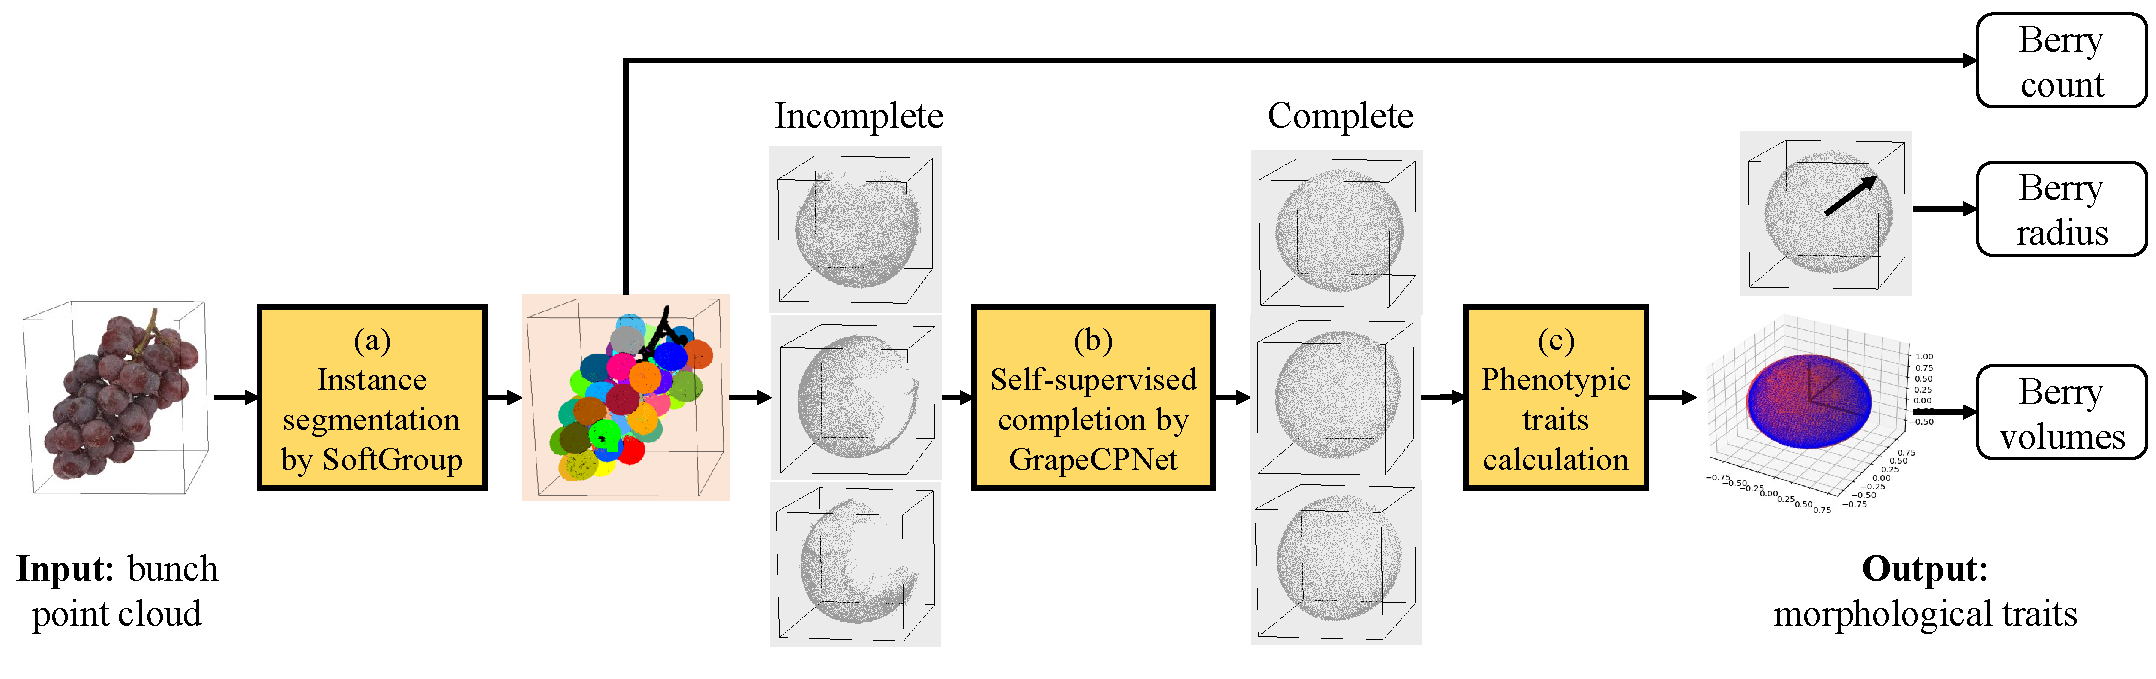
\includegraphics[width=1\textwidth]{figures/Figure1.pdf}
    \caption{Proposed pipeline for grape bunch 3D phenotyping. Taking the bunch point cloud data as input, it is realized through three steps: (1) berry instance segmentation by SoftGroup[32], (2) berry point cloud completion by proposed GrapeCPNet, and (3) phenotypic traits calculation.}
    \label{fig:raw1}
\end{figure}

\subsection{Plant Materials and Point Cloud Acquisition}

\subsubsection{Grape species selection}

To ensure the generality and applicability of the study, this paper considers the sparsity, shape, and color of the bunch, and chooses four common fresh grapes as the experimental materials, which are Red Grape, Green Grape, Kyoho Grape, and Shine-Muscat Grape. 
The characteristics of them are shown in Table~\ref{tlb:1} and the examples are shown in Figure~\ref{fig:raw86}.

% table 1
\begin{table}[h]
    \centering
    \caption{Comparison of the characteristics of the four species of fresh grape}
    \begin{tabular}{cccc}
        \hline
        \textbf{Grape Species} & \textbf{Color} & \textbf{Sparsity} & \textbf{Shape} \\
        \hline
        Red & Purple-red & Sparser & Ellipsoid \\
        Green & Green & Sparse & Ellipsoid \\
        Kyoho & Dark-purple & Dense & Sphere \\
        Shine-Muscat & Green & Very dense & Sphere \\
        \hline
    \label{tlb:1}
    \end{tabular}
\end{table}

% fig.8 + fig.6 -> Fig.2
\begin{figure}[hbt!]
    \centering
    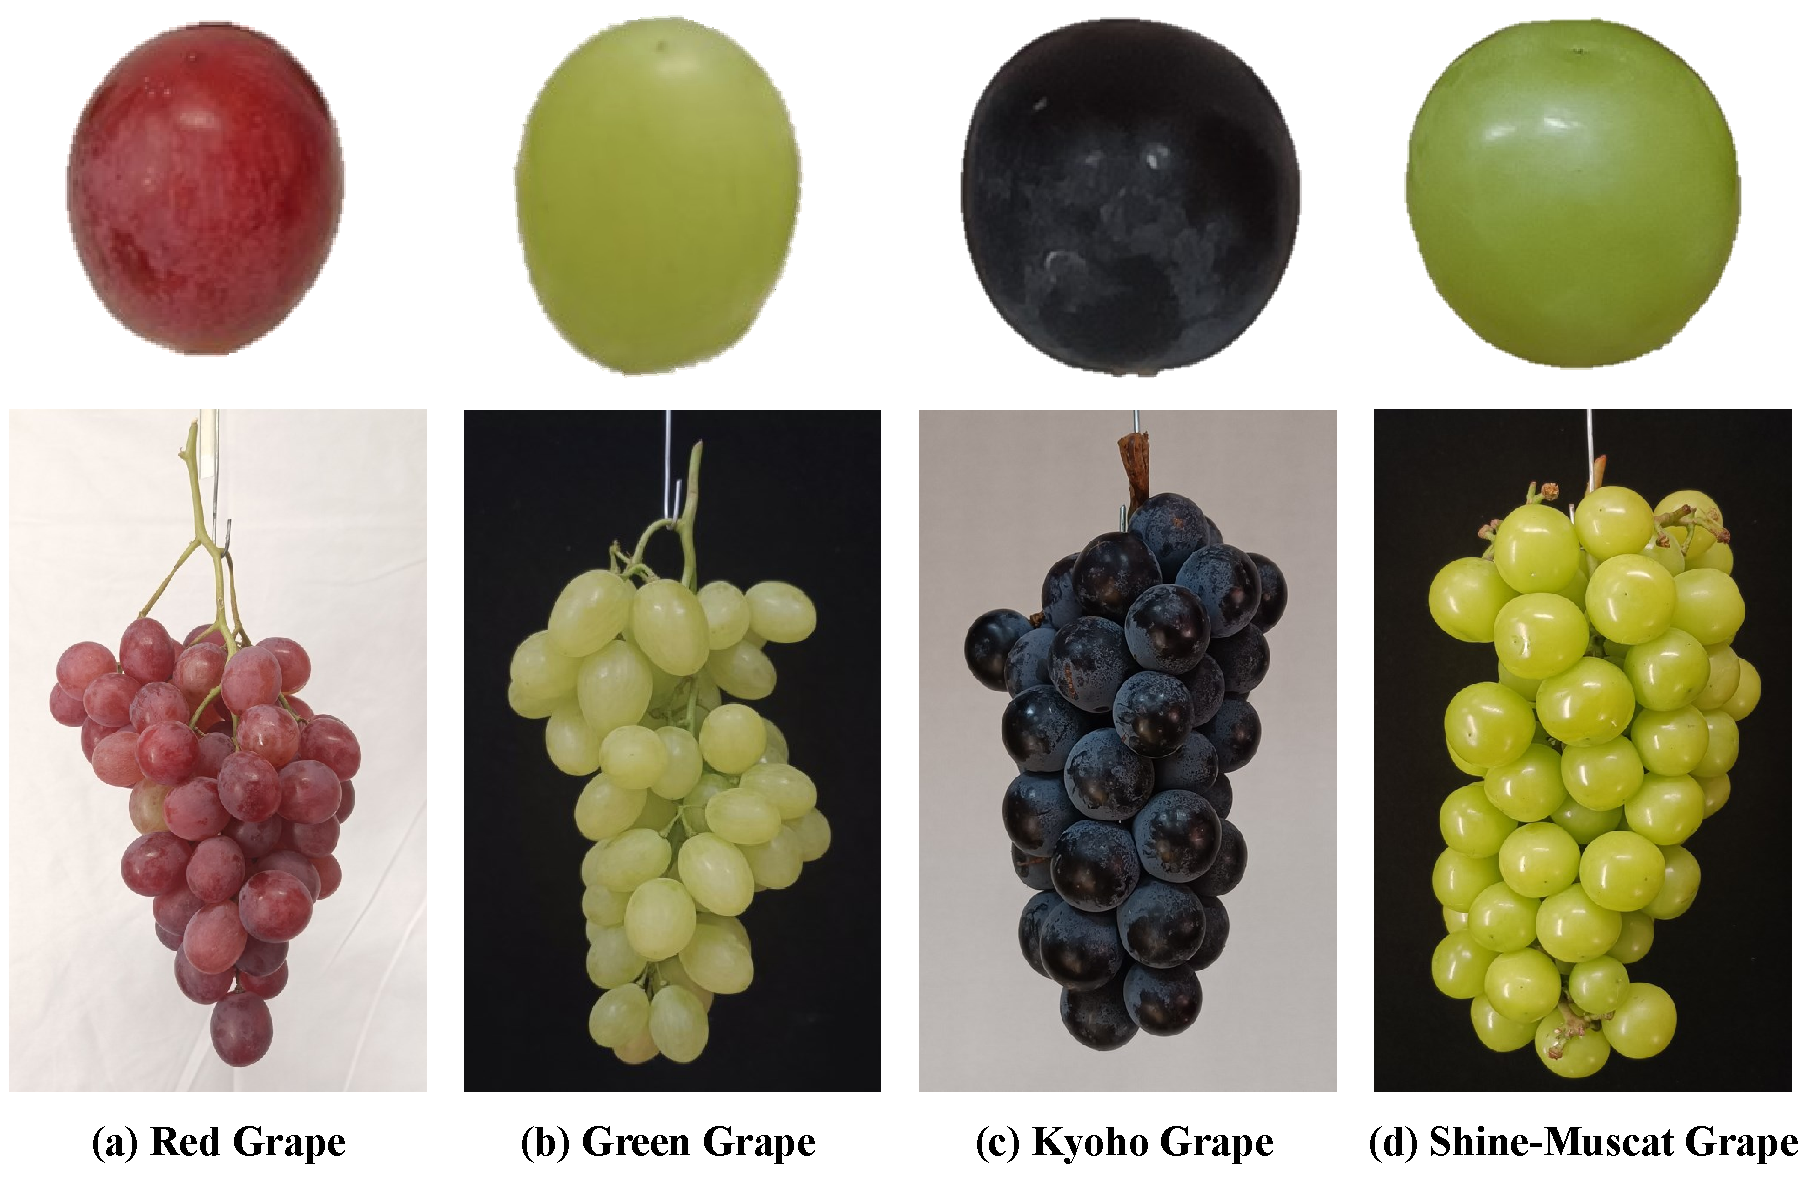
\includegraphics[width=1\textwidth]{figures/Figure2.pdf}
    \caption{Examples of four fresh grape bunches and their berries}
    \label{fig:raw86}
\end{figure}

\subsubsection{3D reconstruction of grape}

In this paper, the multi-view images acquisition and 3D reconstruction by Agisoft Metashape (Agisoft LLC, St. Petersburg, Russia) was used to obtain the 3D point cloud of bunch (Fig.~\ref{fig:raw9}a) and single complete berry (Fig.~\ref{fig:raw9}b). 
Their correspondence of the same berry was also labelled as shown in Figure~\ref{fig:raw9}c

% fig.9
\begin{figure}[hbt!]
    \centering
    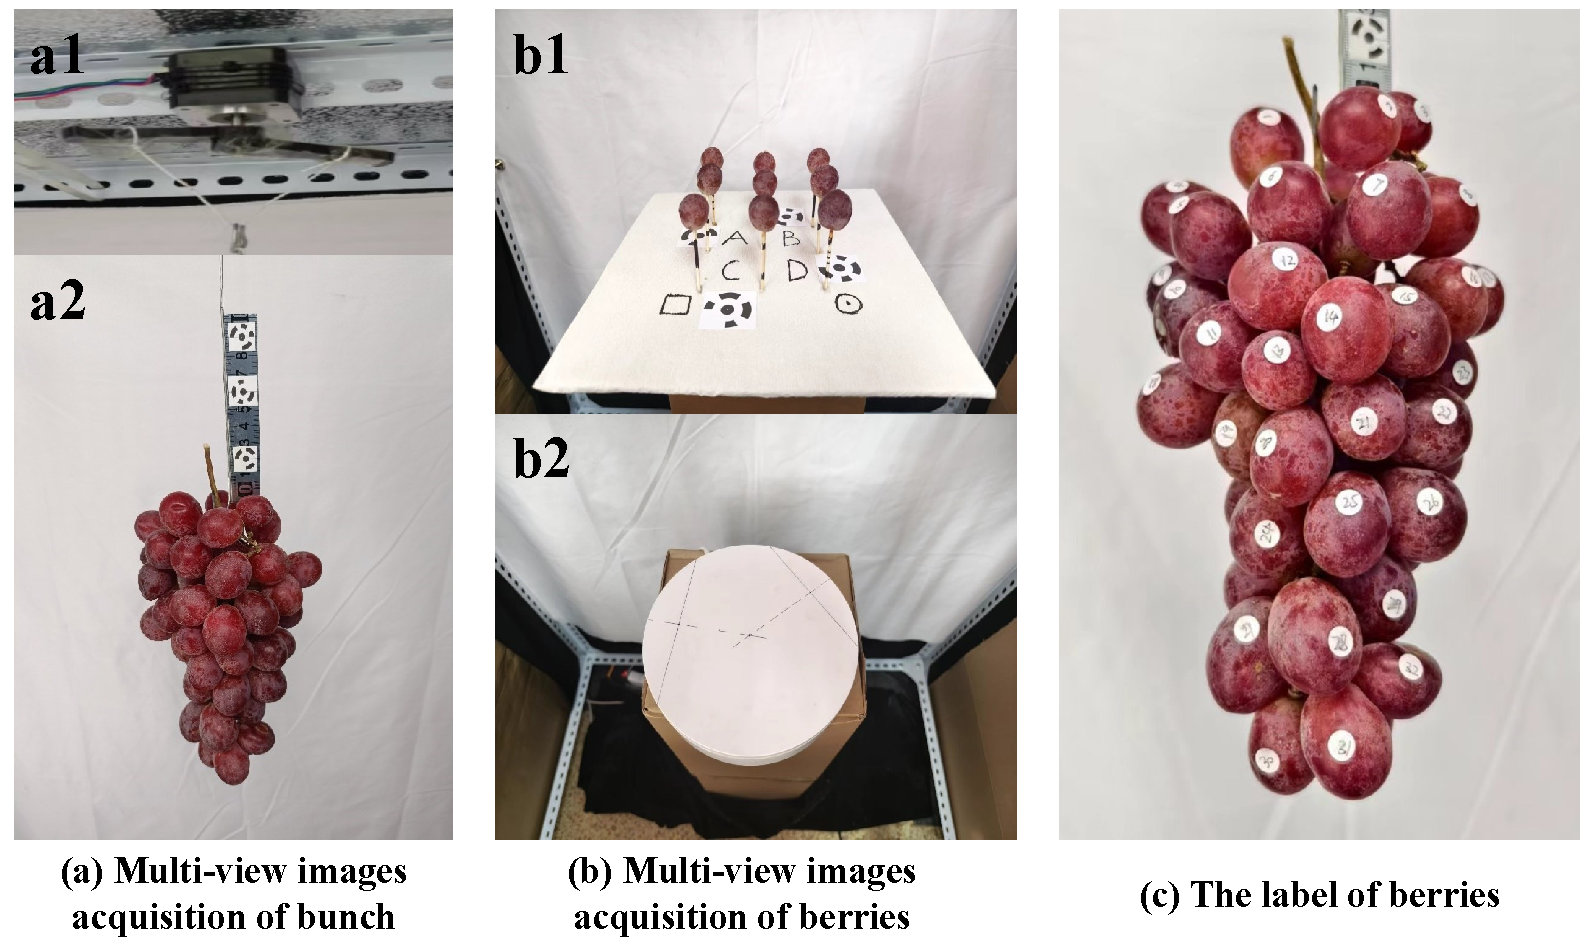
\includegraphics[width=1\textwidth]{figures/Figure3.pdf}
    \caption{Methods for obtaining multi-view images of bunch reconstruction and berry reconstruction, and the example of berry labeling}
    \label{fig:raw9}
\end{figure}

For whole bunch multi-view images acquisition, the device was built as shown in Figure~\ref{fig:raw9}a. 
One grape bunch was hung on the hook which was attached to propellers driven by stepping motors (Fig.~\ref{fig:raw9}a1) that can achieve rotation at a certain speed. 
The entire device was placed in front of a solid-colored backdrop (Fig.~\ref{fig:raw9}a2), and multiple cameras were set up to photograph the bunch from different height angles. 
In addition, a ruler with markers were used for scale correction. 
For single complete berry multi-view images acquisition in batch (Fig.~\ref{fig:raw9}b). 
Nine berries were fixed floating by needle disk (Fig.~\ref{fig:raw9}b1) on a turntable device (Fig.~\ref{fig:raw9}b2). 
The background, cameras, and marker settings are similar to the previous bunch reconstruction. 
The number of reconstructed images and the shooting parameters are selected, as shown in Table~\ref{tlb:2}. 
Examples of the point cloud of bunch, multiple berries, and single complete berries from multiple berries are shown in Figure~\ref{fig:raw10}.

% table 2
\begin{table}[h]
    \centering
    \caption{Comparison of the characteristics of the four species of fresh grape}
    \begin{tabular}{cccc}
        \hline
        \textbf{Object} & \textbf{Shooting distance} & \textbf{Shooting angle} & \textbf{Number of images} \\
        \hline
        Bunch        & 25-60cm & $0^{\circ}$, $\pm 25^{\circ}$, $\pm 45^{\circ}$ & $5 \times 50$ \\
        Single berry & 20-40cm & $-15^{\circ}$, $0^{\circ}$, $25^{\circ}$, $45^{\circ}$ & $4 \times 50$ \\
        \hline
    \label{tlb:2}
    \end{tabular}
\end{table}

% figure 10
\begin{figure}[hbt!]
    \centering
    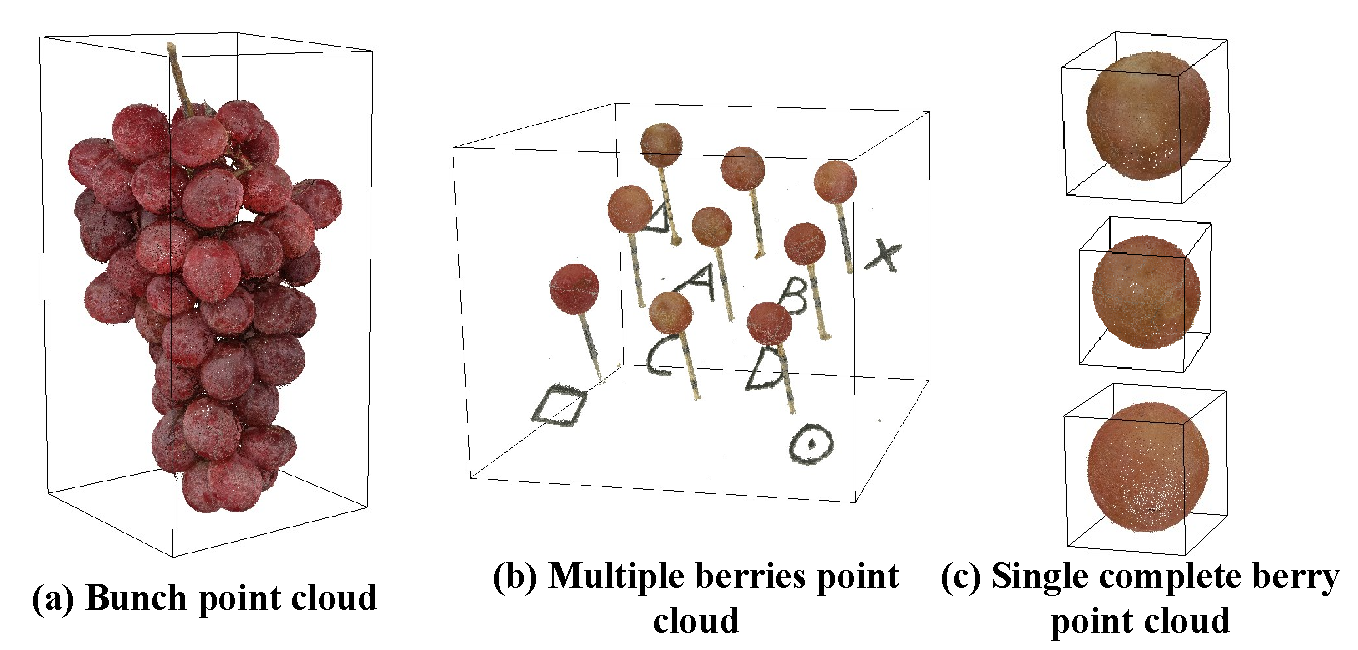
\includegraphics[width=1\textwidth]{figures/Figure4.pdf}
    \caption{Example of point cloud obtained based on multi-view images reconstruction}
    \label{fig:raw10}
\end{figure}

\subsection{Berry Instance Segmentation}

As Figure~\ref{fig:raw1}a, the single-bunch shell point cloud was represented as $P_{bunch}=\{p_i \mid i=1, \cdots, m\}$, where $p_i=(x_i,y_i,z_i)$ denotes a point in 3D space and $m$ denotes the total number of points in the point cloud of the bunch. The bunch point cloud segmentation task expects to segment $P_{bunch}$ into a combination of several individual subsets of the berries point cloud and a subset of the stem point cloud, as shown in Equation~(\ref{eq:1}).

\begin{equation}
P_{bunch} = \sum_{i=1}^{n} P_{berry_{i}} + P_{stem}
\label{eq:1}
\end{equation}

{\raggedright where, $P_{berry_{i}}$ denotes the subset point cloud of the $i^{\text{th}}$ berry in the bunch, $n$ denotes the number of all the berries contained in the bunch, and $P_{stem}$ denotes the set of stem point cloud. 
Meanwhile, each subset $P_{berry_{i}}=\{p_j \mid j=1, \cdots, k\}$ consists of multiple points in 3D space, which can represent the location and morphology of the visible part of the berry within the bunch.}

The task of instance berry segmentation from a bunch is complex. 
As shown in Figure~\ref{fig:raw2}, it involves distinct localization features and complex boundary morphology. 
The distinct localization feature implies that individual berry has more geometrical and morphological details compared to the overall shape of the grape bunch, particularly when the object is a small-sized point cloud [31]. 
The complex boundary morphology arises from berries pressing against each other, resulting in multiple curves with varying connecting depths. 
Therefore, accurate berry instance segmentation requires a model that can both capture detailed geometric features and identify instances at boundary point. 

% figure 2
\begin{figure}[hbt!]
    \centering
    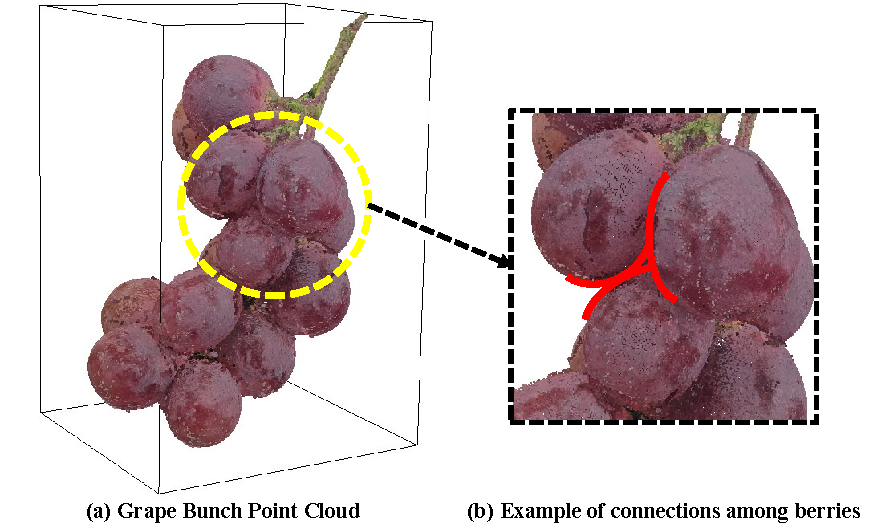
\includegraphics[width=1\textwidth]{figures/Figure5.pdf}
    \caption{Example of berry connection in a bunch (in the case of Red Grape). The red line in the figure shows the characteristics: multiple curves of different depths intersect each other}
    \label{fig:raw2}
\end{figure}

In this paper, SoftGroup [32] was selected for bunch point cloud segmentation by comparing different current deep learning-based point cloud instance segmentation models. 
SoftGroup contains two aspects of design: 
(1) the point-by-point prediction U-Net was used to capture the detailed geometric characteristics between points. 
(2) a threshold score was used to judge the boundary of the point to avoid point category misclassification. 
Therefore, it is suitable for use in a bunch where there is a tight connection boundary among the berries.

In order to train and validate SoftGroup, each berry and stem in the bunch point cloud obtained in
% todo
Section 2.1.2 was labeled at the instance-level (Fig.~\ref{fig:raw11}). 
This paper collected and labeled 8 bunches for each of the four species (total 32 bunches). 
In the sample division, 5 grape bunches of each species (total 20) are randomly selected and used as training samples, the remaining 12 bunches are used for validation.

% figure 11
\begin{figure}[hbt!]
    \centering
    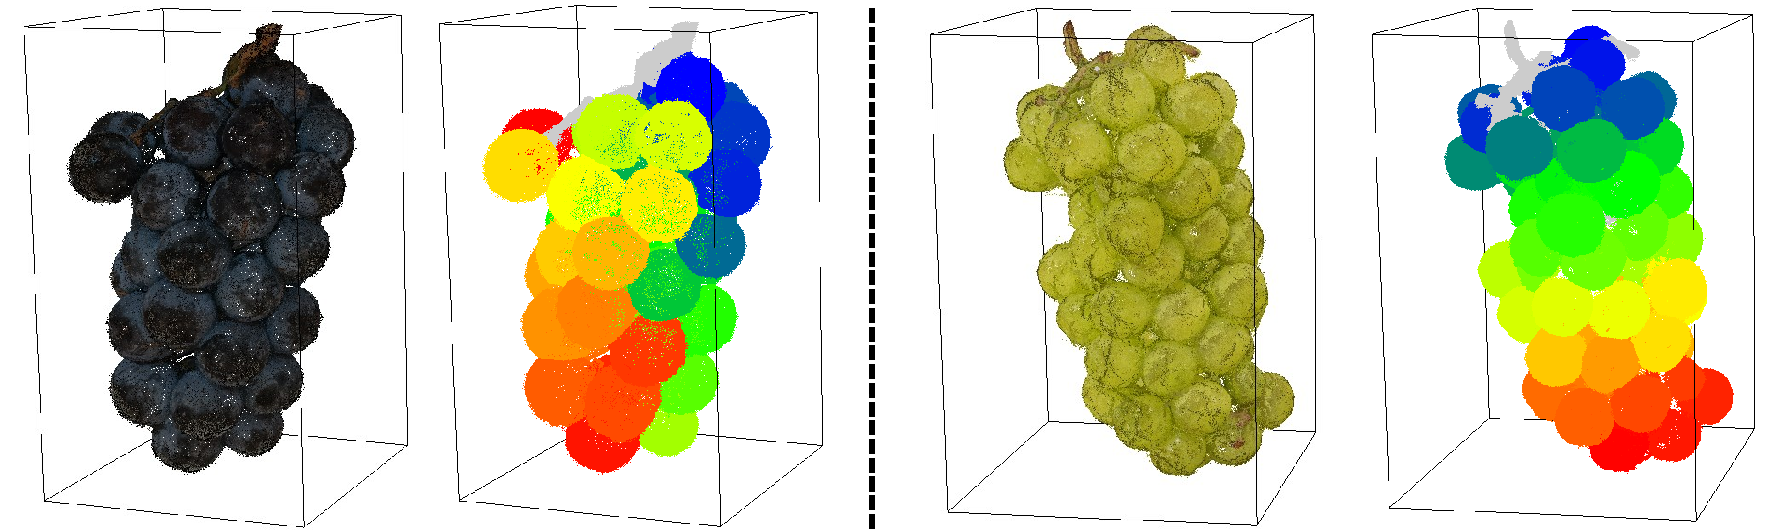
\includegraphics[width=1\textwidth]{figures/Figure6.pdf}
    \caption{Example of instance-level labeling of a bunch point cloud: each berry has a unique instance label, as shown by different colors of point sets}
    \label{fig:raw11}
\end{figure}

\subsection{Self-Supervised Point Cloud Completion}

The self-supervised training-based berry point cloud completion was used to predict their complete 3D model. 
Self-supervised learning is a way of training a model without artificial annotations by using the data itself as truth value to supervise [33]. 
This subsection introduced the self-supervised strategy to generating paired training data without manual annotation and the structure of grape completion network, GrapeCPNet. 
The whole workflow of proposed GrapeCPNet is shown in Figure~\ref{fig:raw3}.

% figure 3
\begin{figure}[hbt!]
    \centering
    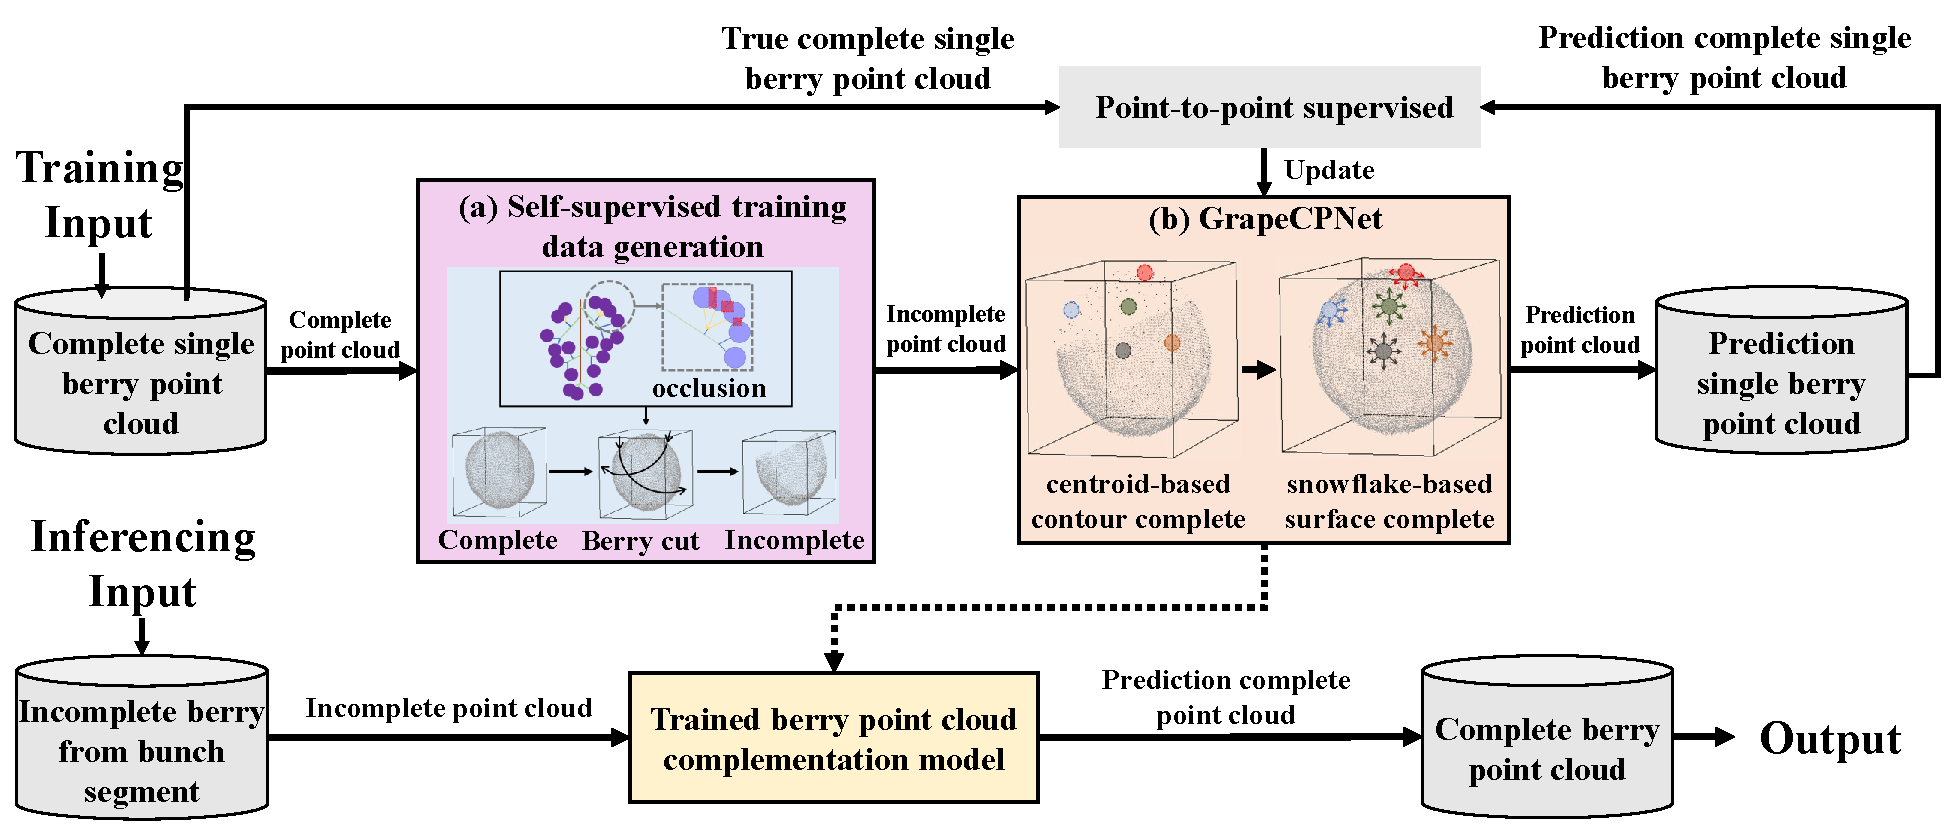
\includegraphics[width=1\textwidth]{figures/Figure7.pdf}
    \caption{Flowchart of the self-supervised berry point cloud completion, including model training and model inferencing (application) phases. In the training phase, the paired incomplete training data was generated from the complete single berry point cloud, then train GrapeCPNet self-supervisely without manual annotation. In the application phase, the incomplete berry point cloud is input into the trained model to obtain a complete prediction berry.}
    \label{fig:raw3}
\end{figure}

\subsubsection{Self-supervised training data generation}

The point cloud completion network often requires the incomplete-complete data pairs of the same object to build a mapping relationship. 
In this paper, the complete grapes were obtained by single berry reconstruction 
%todo
(Section 2.1.2) and were used as ground truth, while the incomplete grapes were cut from the complete grapes following characteristic of occlusion and were used as training inputs. 
This data pair generation strategy saved huge amounts of data annotation. The common incomplete characteristics of the berry are shown in Figure~\ref{fig:raw4}.
Based on the incomplete characteristics, we developed a cutting method for the complete berry point cloud to generate the incomplete berry point cloud.

% figure 4
\begin{figure}[hbt!]
    \centering
    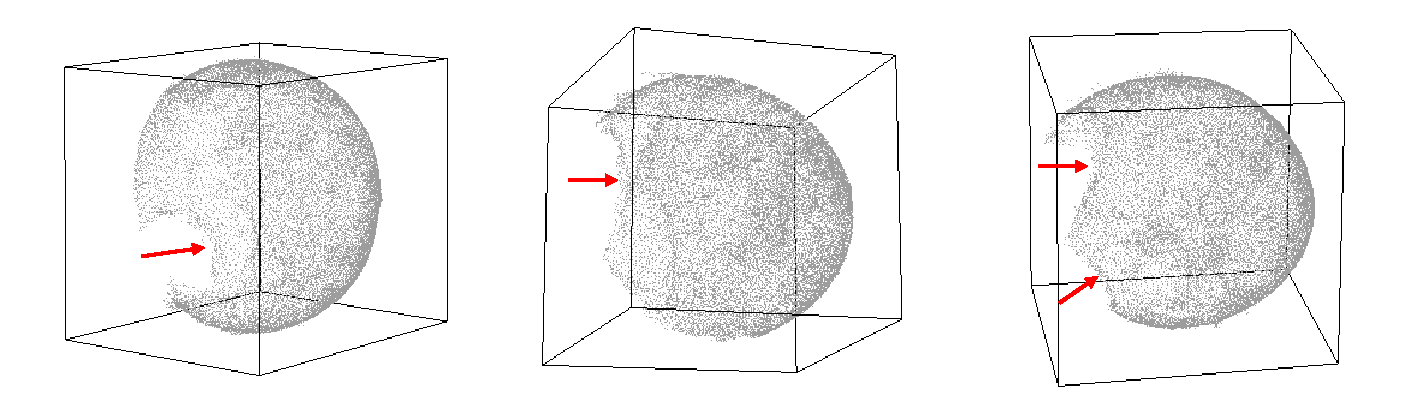
\includegraphics[width=1\textwidth]{figures/Figure8.pdf}
    \caption{Example of different perspectives of an incomplete berry point cloud segmented from the bunch. The edge of the absence shows multiple segments connected by circular curves, as shown by the red arrows}
    \label{fig:raw4}
\end{figure}

This proposed algorithm is shown in Algorithm \ref{alg:1}. 
The inputs include a single complete berry point cloud and the maximum number of cutting area (5 in this paper). 
The output is the cut incomplete berry point clouds. First, the single complete berry point cloud was normalized and centralized (Fig.~\ref{fig:raw12}a). 
Second, randomly pick the integer number of cuts lower than maximum number, in this paper ranging from 1 to 5. 
Then, for each loop of cutting, a 3D sphere model was generated in the space to collide with the berry point cloud, and the collision portion was removed to complete the cutting operation. 
The maximum of center and radius parameters of 3D sphere model were manually set according to berry size. 
In this paper we set maximum 0.75 for center offsets and maximum 0.25 for radius. 
Continue the previous cut looping until meet the cut limits. The cut incomplete berry of each loop was all saved as training data (Fig.~\ref{fig:raw12}b). 

% algorithm 1
\begin{algorithm}
    \caption{The cutting method for generating training data of incomplete berries}
    \label{alg:1}
    \KwData{$P_C$ \tcp{one complete berry point cloud}}
    \KwData{$n$ \tcp{generate incomplete berries number}}
    \KwResult{$P_{\text{output}} = \{P_{o_i} \mid i = 1, \cdots, n\}$ \tcp{incomplete berry point cloud sets} }
    
    $\hat{P_C} \gets Normalize(Translate(P_C))$ \tcp{center to $(0,0,0)$, range to $[-0.5, 0.5]$}
    \For{$i = 0 \to n$}{
        set $m = \text{random}\{1,2,3,4,5\}$ \tcp{cut incomplete single berry $m$ times}
        $P_{o_i} \gets copy(\hat{P_C})$ \tcp{initialize one output}
        \For{$j = 0 \to m$}{
            set $O = \{(x_o, y_o, z_o) \mid x, y, z \in \text{random}[-0.75, 0.75]\}$ \tcp{center variable} 
            set $R = \text{random}[0.25, 0.75]$ \tcp{radius variable}
            set $M_S \gets sphere(O, R)$ \tcp{genreate sphere cut model}
            $P_{o_i} = P_{o_i} - P_{o_i} \cap M_S$ \tcp{remove overlap with cut shpere model}
        }
        $P_{o_i} \in P_{\text{output}}$ \tcp{add to output set}
    }
\end{algorithm}

% figure 12
\begin{figure}[hbt!]
    \centering
    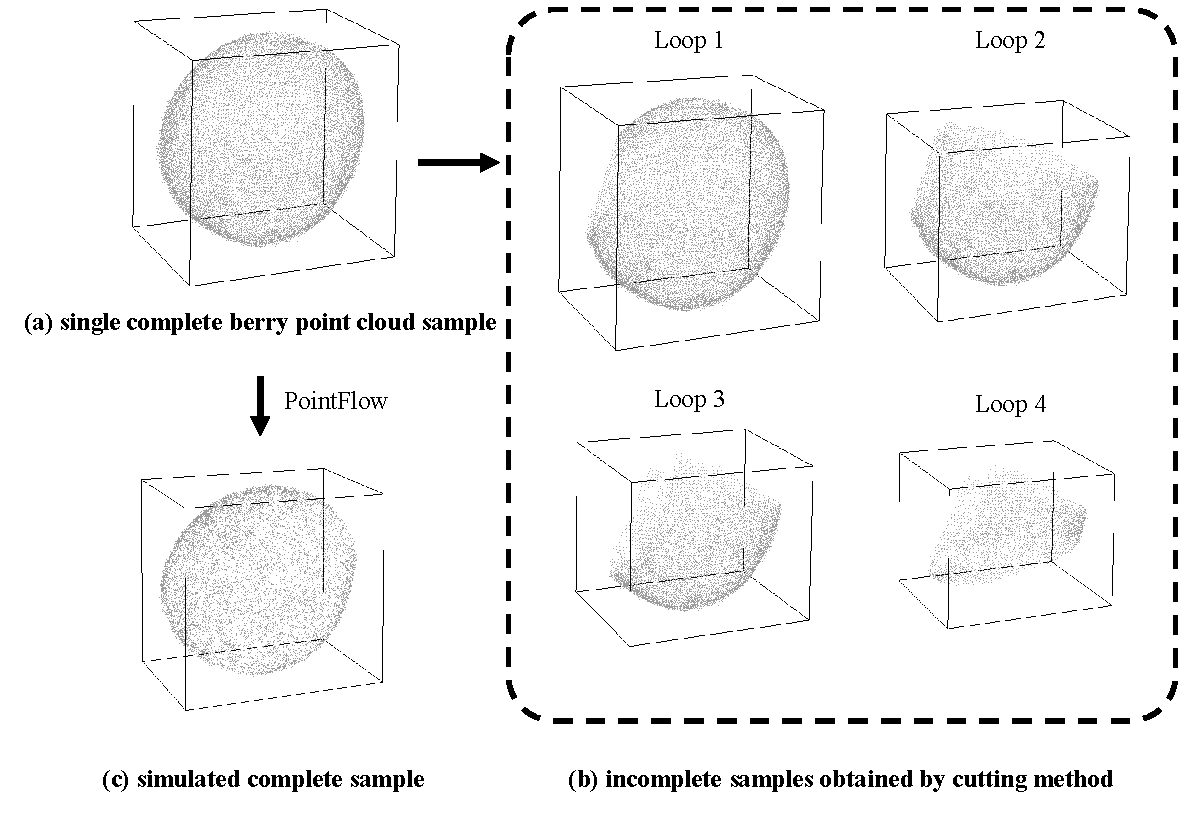
\includegraphics[width=1\textwidth]{figures/Figure9.pdf}
    \caption{Example of dataset composition for the self-supervised training-based method of the berry point cloud completion network.}
    \label{fig:raw12}
\end{figure}

For model training, 36 complete berry are collected for each of the four species of grape (in total 144). 
To further expand the data quantity, based on the single complete berry point cloud obtained by reconstruction, this paper uses the PointFlow [40], a point cloud generation model to generate the simulated samples (Fig.~\ref{fig:raw12}c). 
Then, 500 complete berry point clouds are generated from PointFlow method. 
Thus, a total of 644 complete samples are obtained. 
Each complete berry point cloud has 5 incomplete berry point clouds corresponding to it, and a total of 3220 training data pairs are obtained. 
For the training and testing of the model, this paper divides the dataset according to a ratio close to 7:3, with a total of 450 complete berry point clouds (2250 training data pairs) to train the network and 194 complete berry point clouds (970 testing data pairs) to test.

For the model inference validation, among 12 testing grape bunches of the berry instance segmentation model 
%todo
(Section 2.2), each grape species was randomly selected one bunch (total 4 bunches). 
For each bunch, 27 berries are randomly selected, and finally obtain a total of 108 incomplete berries as the input data for completion network inference validation. 
By checking the labels of these berries, the corresponding single complete berry reconstruction results %todo
(Section 2.1.2 \& Fig.~\ref{fig:raw9}c) were used as ground truth.

\subsubsection{GrapeCPNet structure}

Since the entire contour of the incomplete berry is missing, the model is required to have the ability to predict the incomplete part based on the visible part and make the prediction part fit the real berry surface and avoid detail distortion. 
This paper combines the centroid-based sparse completion structure of PoinTr [35] with the diffusion-based dense completion structure of SnowFlakeNet [36]. 
Based on the characteristics of the berry, it has two parts: contour completion and surface completion. The network structure is shown in Figure~\ref{fig:raw5}.

% figure 5
\begin{figure}[hbt!]
    \centering
    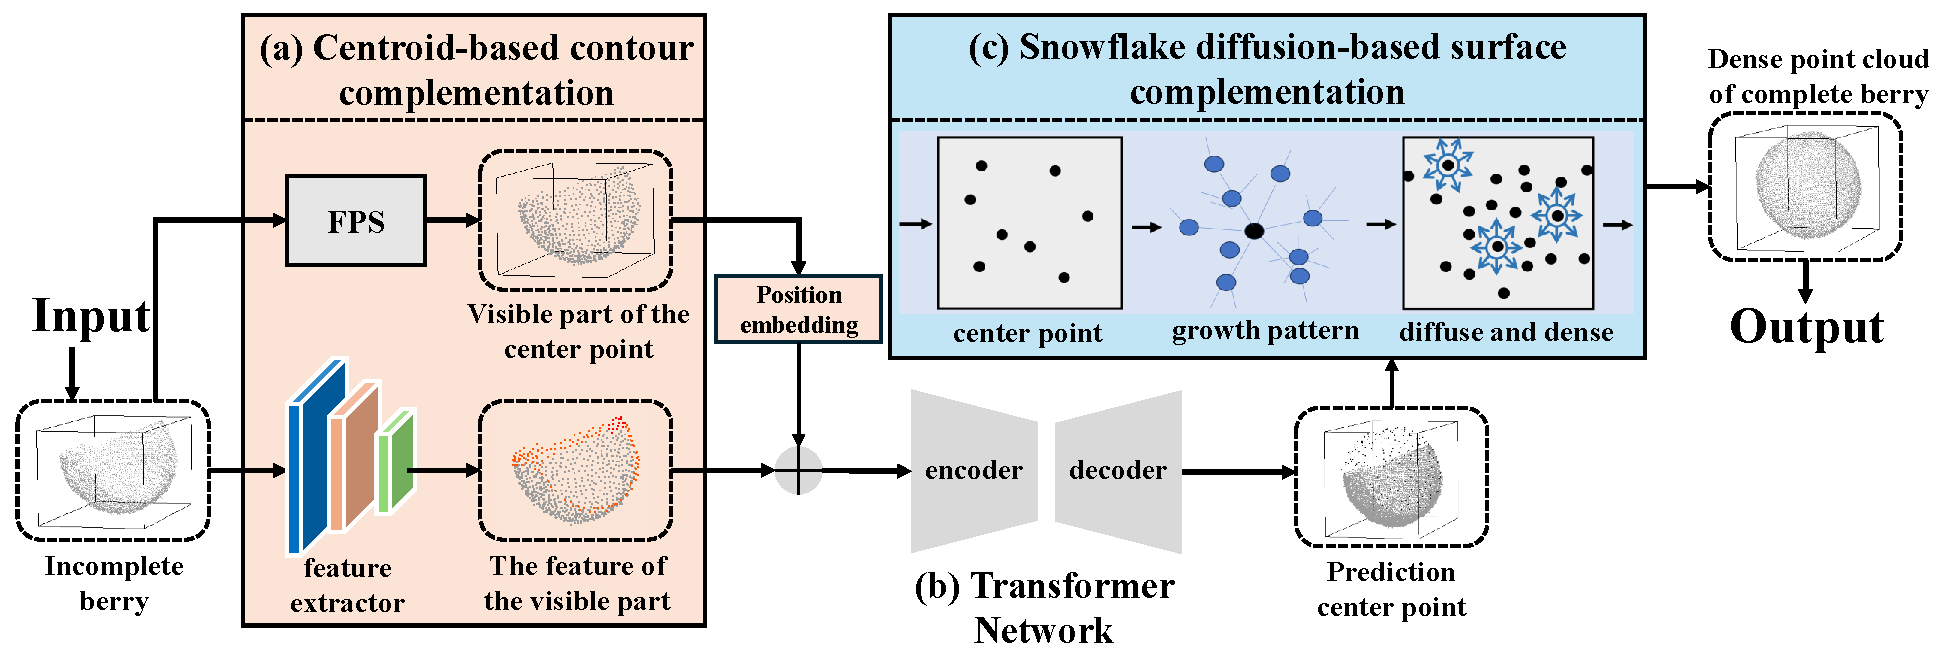
\includegraphics[width=1\textwidth]{figures/Figure10.pdf}
    \caption{GrapeCPNet structure. (a) Centroid-based completion and (b) Transformer network for contour completion of incomplete berry, using sparse point cloud to determine the entire shape; (c) Snowflake diffusion-based completion for dense surface completion to obtain final prediction.}
    \label{fig:raw5}
\end{figure}

{\raggedright\textbf{(1) Centroid-based berry contour completion}}

The visible portion of the incomplete berry belongs to a part of a sphere or ellipsoid, characterized by a distinctly spherical surface. 
In addition, the point cloud is unstructured data, unstructured and dense, resulting in features that cannot be effectively extracted. 
Based on the above analysis, this paper utilizes the centroid set of the visible part to infer the centroid set of the invisible part. 
Specifically, GrapeCPNet uses centroid-based feature extraction in PoinTr [35] to accomplish berry point cloud contour completion. The process is described below: 

Assume that the set of incomplete berry point cloud as input to the network is represented as $P_{partial}=\{p_i \mid i=1, \cdots, m \}$, where $p_i=(x_i,y_i,z_i)$ denotes a point in 3D space and $m$ denotes the number of points. 
The berry point cloud completion task aims to output the complete berry point set $P_{complete}=\{p_i \mid i=1, \cdots, n\}$, where $n$ denotes the number of points of the output, and $n > m$, thereby it can represent the complete 3D morphology of the berry.

After the incomplete berry point cloud set $P_{partial}=\{p_i \mid i=1,\cdots,m\}$ was fed into the network, it was firstly down-sampled to a fixed number of points $M$ ($M$ is often less than $m$, in this paper, $M$ is set to 2048) through the farthest point sampling (FPS) to obtain the center point set $P_{partial-center}=\{p_i \mid i=1, \cdots, M\}$ of the visible part of the berry. 
This set was used as a ``representative'' to avoid huge computational effort while characterizing the complete morphology of the visible part.

Then, the 3D convolutional neural networks DGCNN [37] and MLP [38] are used to obtain the local structural features of each point $p_i$ in the center point set, as shown in Equation~(\ref{eq:2}).

\begin{equation}
    F_i = F_{i}^{'} + \varphi(p_i)
    \label{eq:2}
\end{equation}

{\raggedright where, $F_{i}^{'}$ denotes the feature around $p_i$ obtained by DGCNN, which is the local feature of the point in the point cloud; and $\varphi(p_i)$ denotes the position information of $p_i$ obtained by MLP, which is the global feature of the point.}

Finally, since the $\varphi = \{ \varphi(p_i) \mid i=1, \cdots, M \}$ contains the relative position information of each point, it can be used as the position embedding and the serialized feature $F = \{F_i \mid i=1, \cdots, M \}$ was fed into the geometrically-aware Transformer [39] based encoder. 
The process is Equation~(\ref{eq:3}).

\begin{equation}
    V = T_e(F)
    \label{eq:3}
\end{equation}

{\raggedright where, $T_e$ denotes the encoder of the Transformer and $V=\{V_i |i=1, \cdots, M\}$ denotes the encoded feature. 
Next, the predicted centroid point set of the missing part was output by the decoder, and the process as Equation~(\ref{eq:4}).}

\begin{equation}
    P_{pred-center} = T_d(V)
    \label{eq:4}
\end{equation}

{\raggedright where, $T_d$ denotes the decoder of the Transformer, $P_{pred-center}=\{p_i \mid i=1,\cdots,N\}$ denotes the predicted centroid point set, and $N$ denotes the number of points in the set. 
Through the above steps, the set of center points of the complete berry can be initially obtained, which was the result of sparse contour completion.}

{\raggedright\textbf{(2) Snowflake diffusion-based berry surface completion}}

The results of the contour completion can determine the overall 3D morphology, however, the density of this sparse point cloud requires the model can capture the detail surface geometry changes between points to avoid distortion. 
Therefore, this paper utilizes the snowflake diffusion-based generation idea to regard each point in the contour completion as the center point of the local region. 
It diffuses based on the centroid points and generates further at the generated location, densification by point-to-point splitting. 
Specifically, as follows:

First, GrapeCPNet sets each point $p$ of the sparse complement $P_{pred-center}=\{p_i \mid i=1,\cdots,N\}$ as a ``seed point''. 
Then, $P_{pred-center}$ was fed into multiple SPD [36] connected serially of SnowFlakeNet, which are used to realize point splitting and generation. 
On the one hand, the SPD diffuses from the center point in a tree structure around, revealing the detailed geometric structure of the local region. 
This method effectively represents the surface geometric features composed between the points in the localized region of the berry. 
On the other hand, the iteration of multiple point splitting steps delivers information from each one to the next one. 
This approach effectively characterizes the curvature changes on the surface of the berry. The process is Equation~(\ref{eq:5}).

\begin{equation}
    P_{i+1} = SPD(P_i)
    \label{eq:5}
\end{equation}

{\raggedright where, $P_i$ denotes the input point cloud of the $i^{\text{th}}$ SPD, $P_{i+1}$ denotes the output point cloud of the $(i+1)^{\text{th}}$ SPD, and $P_0=P_{pred-center}$. 
In this paper, when $i=2$ (an empirical value), the final predicted dense point cloud on the surface of the complete berry $P_3=P_{complete}$ was output and $P_{complete}=\{p_i \mid i=1,\cdots,n\}$.}

Through the above two steps, the complete 3D point cloud model of the berry can be obtained after contour completion and surface completion of GrapeCPNet.

\subsection{Phenotypic Traits Calculation and Validation}

To describe the 3D morphology of berries, this paper used ellipsoidal surface fitting with three axes, for the completed berry point cloud (Fig.~\ref{fig:raw7}).

% figure 7 -> removed

Suppose the point cloud of the complete berry is denoted as $P_{complete}=\{P_i \mid i=1, \cdots,n\}$, where $p_i=(x_i,y_i,z_i)$ denotes a point in the 3D space, and $n$ denotes the number of points. 
In this paper, it is fitted to an ellipsoid surface with three unequal long axes by the least squares method, and the function is shown in Equation~(\ref{eq:6}).

\begin{equation}
    \frac{(x-x_0)^2}{a^2} + \frac{(y-y_0)^2}{b^2} + \frac{(z-z_0)^2}{c^2} = 1
    \label{eq:6}
\end{equation}

{\raggedright where, $(x,y,z)$ denotes a point on the ellipsoid surface, $(x_0,y_0,z_0)$ denotes the coordinates of the ellipsoid center point, and $a$, $b$, $c$ are the half-long, half-middle, and half-short axes, respectively (assuming that $a>b>c>0$). }

Thus, the values of $a$, $b$, $c$ can represent the berry radius parameters. 
At the same time, the volume of the berry can be calculated as shown in Equation~(\ref{eq:7}).

\begin{equation}
    V=\frac{4}{3} \pi a b c
    \label{eq:7}
\end{equation}

In order to validate the accuracy of extracted morphological traits, those 12 validation bunches in %todo
Section 2.2 were continuously used after instance berry segmentation and berry completion. 
The radius and volume of the 108 samples are calculated. 
For ground truth measurement, instead of using manual measurement, which has multiple artificial errors in obtaining the true values of actual radius and volume. 
This paper used the correspond individual complete berry as the ground truth and applied the same method for the radius and volume calculations. 

\subsection{Evaluation Metrics}

In this paper, the evaluation metrics for the bunch segmentation, the berry completion, the effectiveness of the number of berries counting, and the calculation of radius and volume in the acquisition of 3D phenotypic parameters are as follows.

\subsubsection{Berry instance segmentation}

In this paper, we use the format of SoftGroup [32] that is consistent with the S3DIS dataset [41] and use the average precision AP [32] as the evaluation metric for berry instance segmentation. In the threshold setting, the average of the APs with selected the IoU (Intersection over Union) from 50\% to 95\% in steps of 5\% is noted as AP@50:5:95.

\subsubsection{Berry self-supervised completion}

In this paper, we use the format of PoinTr [35] that is consistent with the PCN dataset [42] and use the chamfer distance (CD-distance) and F-Score to measure the effect of berry completion. 
For each sample, the chamfer distance $d_CD$ between the predicted point set $P$ and the true point set $G$ is calculated as shown in Equation~(\ref{eq:8})

\begin{equation}
    d_{CD}(P, G) = \frac{1}{|P|} \sum_{p \in P} \min_{g \in G} \|p - g\|_2^2 + \frac{1}{|G|} \sum_{g \in G} \min_{p \in P} \|g - p\|_2^2
    \label{eq:8}
\end{equation}

{\raggedright where, $|P|$ denotes the number of points of $P$, $|G|$ denotes the number of points of $G$, and $\|p - g\|$ denotes the distance between $p$ and $g$. 
It can be seen that the chamfer distance represents the sum of the average closest distance from the point in $P$ to the point in $G$ and the average closest distance from the point in $G$ to the point in $P$. Where the L1 norm is used to calculate the closest distance between two points.}

In addition, F-Score measures the similarity between $P$ and $G$ by the harmonic mean between Precision and Recall. 
On the one hand, Precision counts the percentage of the number of points of the prediction within a certain distance from the truth point, which represents the accuracy of the prediction;
on the other hand, Recall counts the percentage of the number of points of the truth point within a certain distance from the prediction point, which represents the completeness of the prediction. Specifically, as follows.


\begin{align}
    \text{Precision}(d) &= \frac{1}{|P|} \sum_{p \in P} \left[ \min_{g \in G} \|p - g\| < d \right] \tag{9}\\
    \text{Recall}(d) &= \frac{1}{|G|} \sum_{g \in G} \left[ \min_{p \in P} \|g - p\| < d \right] \tag{10}\\
    F\text{-Score}(d) &= \frac{2 \times \text{Precision}(d) \times \text{Recall}(d)}{\text{Precision}(d) + \text{Recall}(d)} \tag{11}
\end{align}

{\raggedright where, Precision$(d)$ and Recall$(d)$ in (11) denote the Precision and Recall computed under the distance threshold $d$, respectively, and $d$ is set to $0.01$ in the PCN data format. 
From the above Equation, the higher the F-Score indicates that the two point sets are more similar.}

In addition, in order to verify the efficiency of GrapeCPNet, other classical point cloud completion networks, including PoinTr, SnowFlakeNet, TopNet [43], and GRNet [44] are selected as comparison algorithms. 

\subsubsection{Phenotypic traits calculation}

In order to evaluate the efficiency of the number of berry statistics and the calculation of berry radius and volume, the MAE (Mean Absolute Error) and the coefficient of determination $R^2$ (R-Square) are used to calculate the error between the prediction value and the true value of the sample.

\begin{align}
    \text{MAE} &= \frac{1}{m} \sum_{i=1}^{m} |y_i - \hat{y}_i| \tag{12}\\
    R^2 &= 1 - \frac{\sum_{i} (\hat{y}_i - y_i)^2}{\sum_{i} (\bar{y}_i - y_i)^2} \tag{13}
\end{align}

{\raggedright where, $m$ is the number of samples, $y_i$ is the true value of the $i^{\text{th}}$ sample, $\hat{y}_i$ is the prediction value, and $\bar{y}_i$ represents the mean of all true values. 
It can be seen that the lower the MAE, the closer the prediction value is to the true value, and the value of $R^2$ ranges from 0 to 1, and the closer it is to 1 means that the prediction value is better fitted.}

\section{Results}

In order to validate the efficiency of the method proposed in this paper, the experiments are conducted on each component separately, including the result of bunch point cloud segmentation, the result of berry point cloud completion based on self-supervised training, and the result of phenotypic parameters acquisition.

\subsection{Berry Instance Segmentation Results}

Bunch point cloud segmentation is mainly realized based on SoftGroup, a point cloud segmentation network. 
This paper calculates the segmentation results for the berry instances and stem instances using the dataset introduced in 
%todo
Section 2.2 and the evaluation metrics in Section 2.5.1, as shown in Table~\ref{tlb:3}.

% table 3
\begin{table}[h]
    \centering
    \caption{Instance berry segmentation results from whole bunch}
    \begin{tabular}{ccc}
        \hline
        \textbf{Model} & \textbf{Class} & \textbf{AP@50:5:95} \\
        \hline
        \multirow{2}{*}{SoftGroup \citep{vu_softgroup_2022}} & Berry & 0.995 \\
        \cline{2-3}
        & Stem & 0.941 \\
        \hline
    \end{tabular}
\end{table}

As can be seen from Table~\ref{tlb:3}, the AP value of the point cloud instance segmentation for the berry category is over 99\%, which shows a high accuracy of the berry segmentation from the bunch. The visualization results of four fresh grapes for bunch point cloud segmentation using SoftGroup are shown in Figure~\ref{fig:raw13}.

% figure 13
\begin{figure}[hbt!]
    \centering
    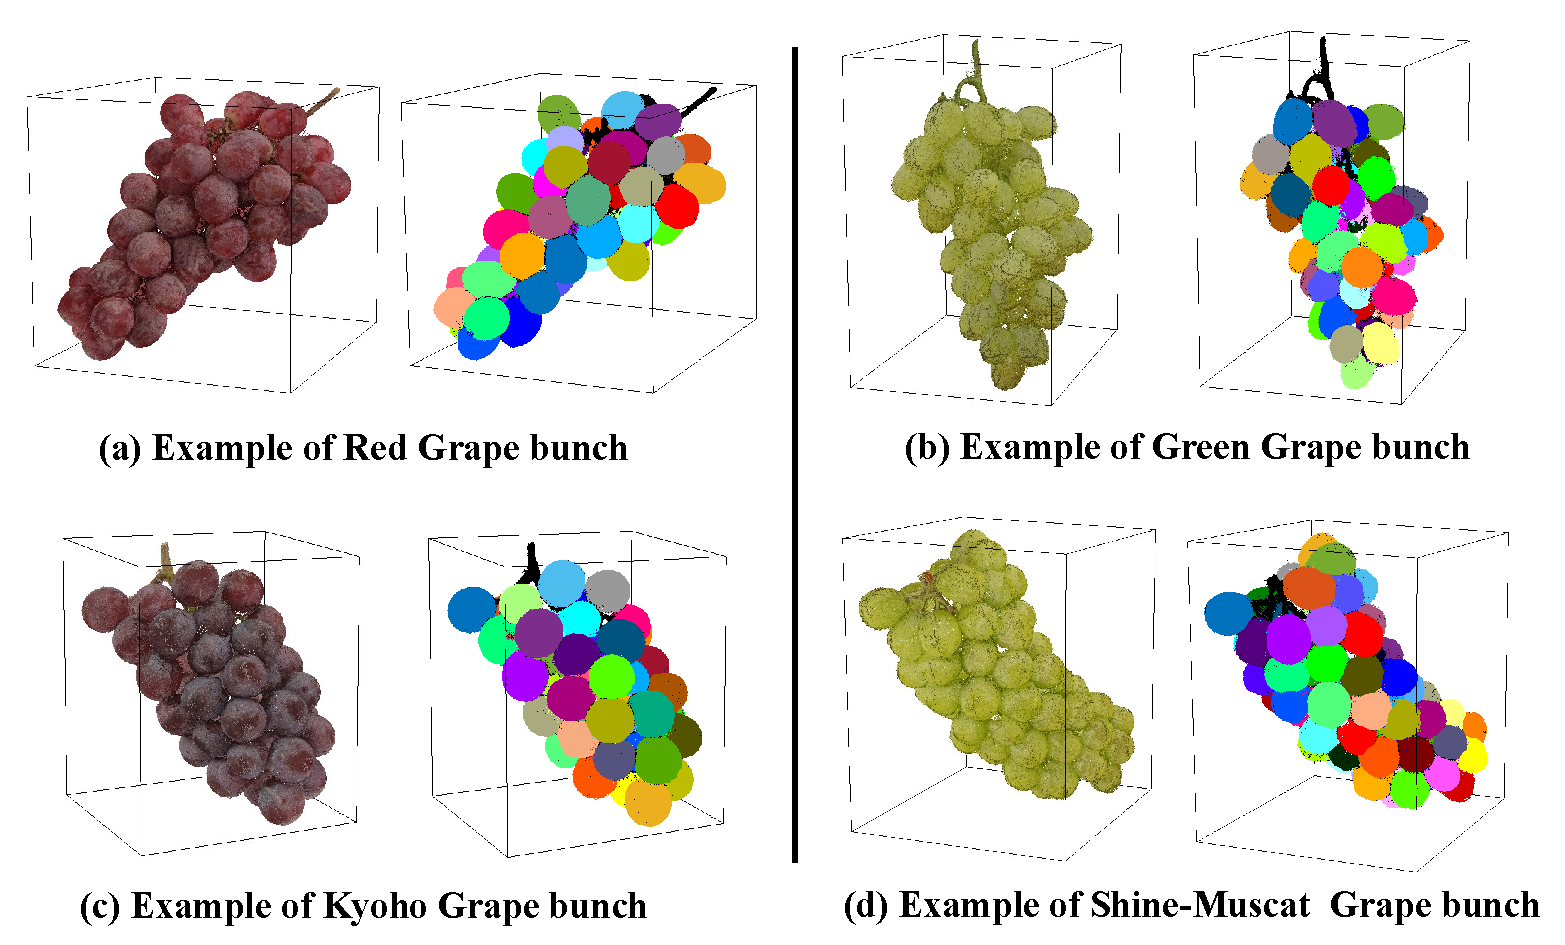
\includegraphics[width=1\textwidth]{figures/Figure11.pdf}
    \caption{Segmentation results of the bunch of four species of fresh grape, the stems point cloud and the noise point cloud are set to black, and the different color point sets indicate the point clouds of different berry instances obtained.}
    \label{fig:raw13}
\end{figure}

\subsection{Berry Self-Supervised Completion Results}

The berry point cloud completion experiments are divided into two parts according to the different phases of the network: the results of the self-supervised training experiments and the results of the practical application experiments.

(1) In the training phase, the incomplete-complete pair of the point cloud of berry is obtained by the cutting method to train the network. 
The samples are divided into the training set and the testing set. Therefore, in order to verify the efficiency of berry point cloud completion in the training phase, experiments are conducted as ``Test''.

(2) In the application phase, the incomplete berries segmented from the bunch are complemented based on the trained berry point cloud completion model. 
Therefore, in order to verify the efficiency of berry point cloud completion in practical applications, experiments are conducted as ``Inference''. 


Meanwhile, since the point cloud obtained after berry picking is used as the ground truth, the point cloud alignment is performed to calculate evaluation metrics of the predicted complete berry point cloud with the ground truth.
The experimental results of comparing to other point cloud completion algorithms are shown in Table~\ref{tlb:4}. 
GrapeCPNet achieves the best results under the self-supervised training method in both the training phase and the application phase, better than the other comparative algorithms. 
The visualization of using GrapeCPNet to complement the incomplete berry segmented from the bunch in the application phase is shown in Figure~\ref{fig:raw14}.

% table 4
\begin{table}[h]
    \centering
    \caption{Experimental results of different completion networks based on self-supervised training for berry point cloud}
    \begin{tabular}{cccccc}
        \hline
        \textbf{Model} & \textbf{DataSet} & \textbf{CD-distance $\downarrow$} & \textbf{Precision $\uparrow$} & \textbf{Recall $\uparrow$} & \textbf{F-score $\uparrow$} \\
        \hline
        \multirow{2}{*}{PoinTr} & Test & 9.036 & 0.721 & 0.705 & 0.713 \\
        \cline{2-6}
        & Inference & 10.542 & 0.623 & 0.601 & 0.612 \\
        \hline
        \multirow{2}{*}{SnowFlakeNet} & Test & 11.235 & 0.512 & 0.534 & 0.521 \\
        \cline{2-6}
        & Inference & 12.384 & 0.415 & 0.423 & 0.419 \\
        \hline
        \multirow{2}{*}{TopNet} & Test & 23.019 & 0.201 & 0.200 & 0.201 \\
        \cline{2-6}
        & Inference & 31.88 & 0.155 & 0.154 & 0.154 \\
        \hline
        \multirow{2}{*}{GRNet} & Test & 19.24 & 0.402 & 0.392 & 0.397 \\
        \cline{2-6}
        & Inference & 21.25 & 0.365 & 0.363 & 0.364 \\
        \hline
        \multirow{2}{*}{GrapeCPNet (\textbf{Ours})} & Test & \textbf{8.315} & \textbf{0.729} & \textbf{0.772} & \textbf{0.751} \\
        \cline{2-6}
        & Inference & \textbf{9.158} & \textbf{0.685} & \textbf{0.696} & \textbf{0.689} \\
        \hline
    \end{tabular}
\end{table}

% figure 14
\begin{figure}[hbt!]
    \centering
    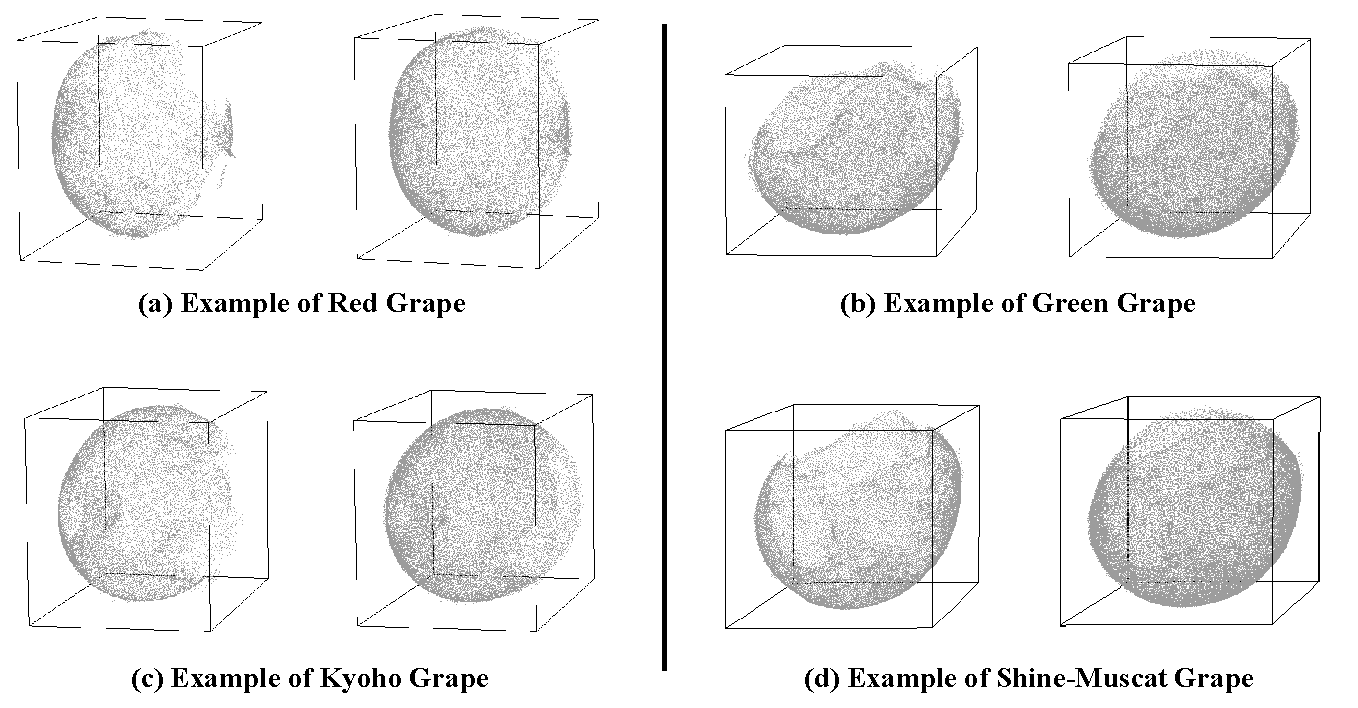
\includegraphics[width=1\textwidth]{figures/Figure12.pdf}
    \caption{Example of four fresh grape berry point cloud completion results: in each block, the left side shows the incomplete berry point cloud obtained from the segmentation of the bunch, and the right side shows the completion results using GrapeCPNet under the self-supervised training-based method.}
    \label{fig:raw14}
\end{figure}

In addition, the results of the ``Inference'' experiments are worse than those of the ``Test'' experiments for two main reasons.
First, there are differences between the dataset of the training phase and the application phase of self-supervised training, resulting in a loss of accuracy in the application of the model. 
In addition, when evaluating the actual application efficiency of the model, the true value of the reconstructed complete point cloud of a single berry and the prediction value of the complemented point cloud suffer from the loss of accuracy when they are aligned.
Through the above results, the experiments of berry point cloud completion based on self-supervised training reflected the efficacy of GrapeCPNet, meanwhile, this paper further validated the efficacy of the 3D phenotypic parameters acquisition of grape by the proposed method.

\subsection{Phenotypic Traits Calculation Results}

Based on the method in this paper, the bunch point cloud is used as input, and the acquired 3D phenotypic parameters are the final output, which mainly contains two parts: the bunch-level phenotypic parameters and the berry-level phenotypic parameters.
In this paper, experiments are conducted to calculate berry radius and volume with the dataset in the evaluation metrics in 
%todo
Section 2.5.3.
The radius parameters are calculated by fitting the berry to the surface of an ellipsoid, as shown in Figure~\ref{fig:raw16}.

% figure 16
\begin{figure}[hbt!]
    \centering
    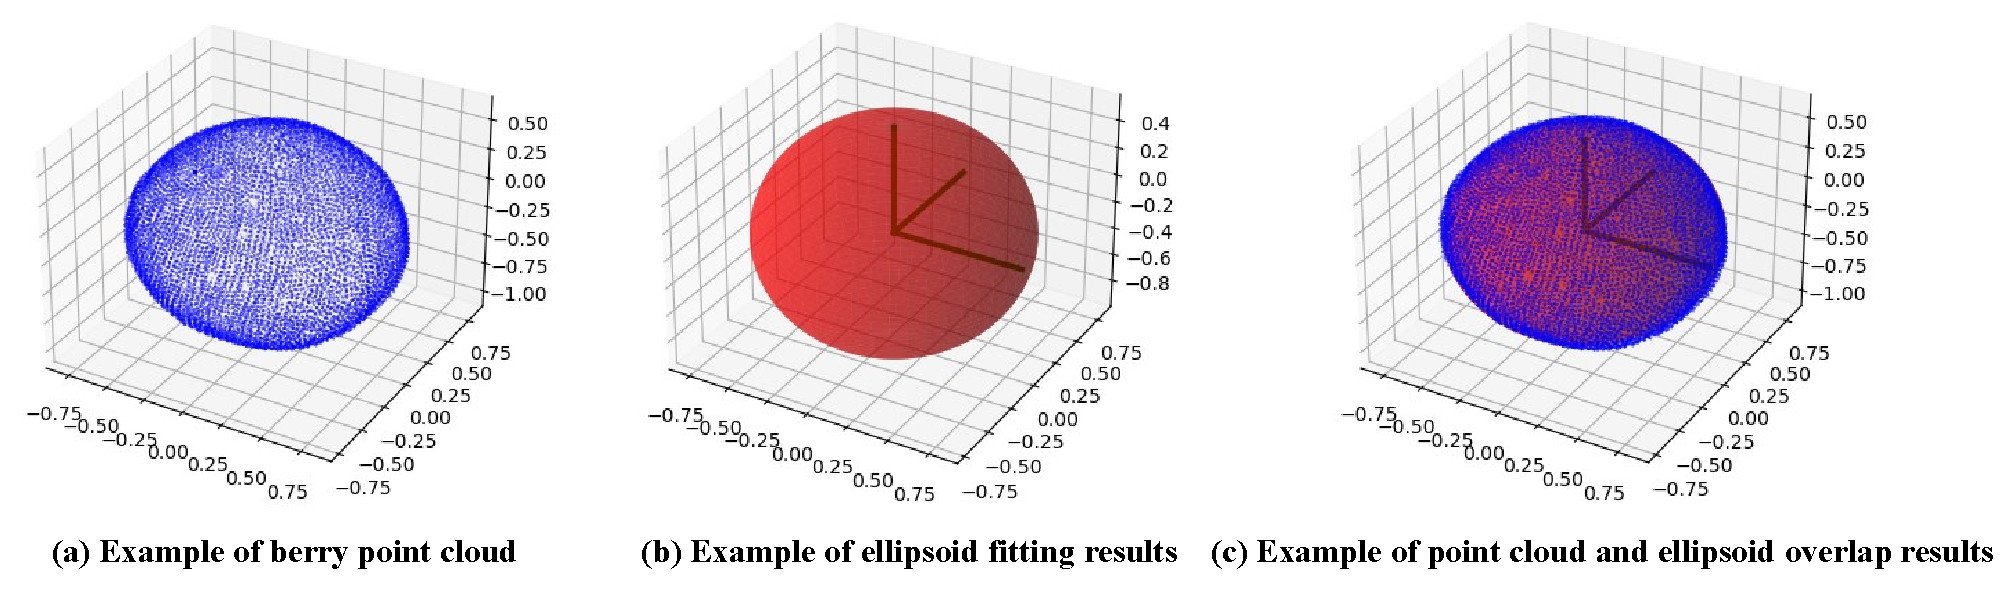
\includegraphics[width=1\textwidth]{figures/Figure13.pdf}
    \caption{Example of visualization of the predicted complete berry point cloud fitted to the surface of an ellipsoid.}
    \label{fig:raw16}
\end{figure}

Three lengths of the radius of the berry can be obtained by fitting the predicted point cloud of the complete berry shell to the surface of an ellipsoid. 
Meanwhile, the point cloud data acquisition method in 
%todo
Section 2.1.2 can translate the scale of the point cloud space to the real world, so as to get the real radius length of the berry.
Because of the large difference between the ratio of the long and short axis of different species, this paper conducted experiments on the calculation of the axis length of four species respectively, as shown in Figure~\ref{fig:raw17}.

% figure 17
\begin{figure}[hbt!]
    \centering
    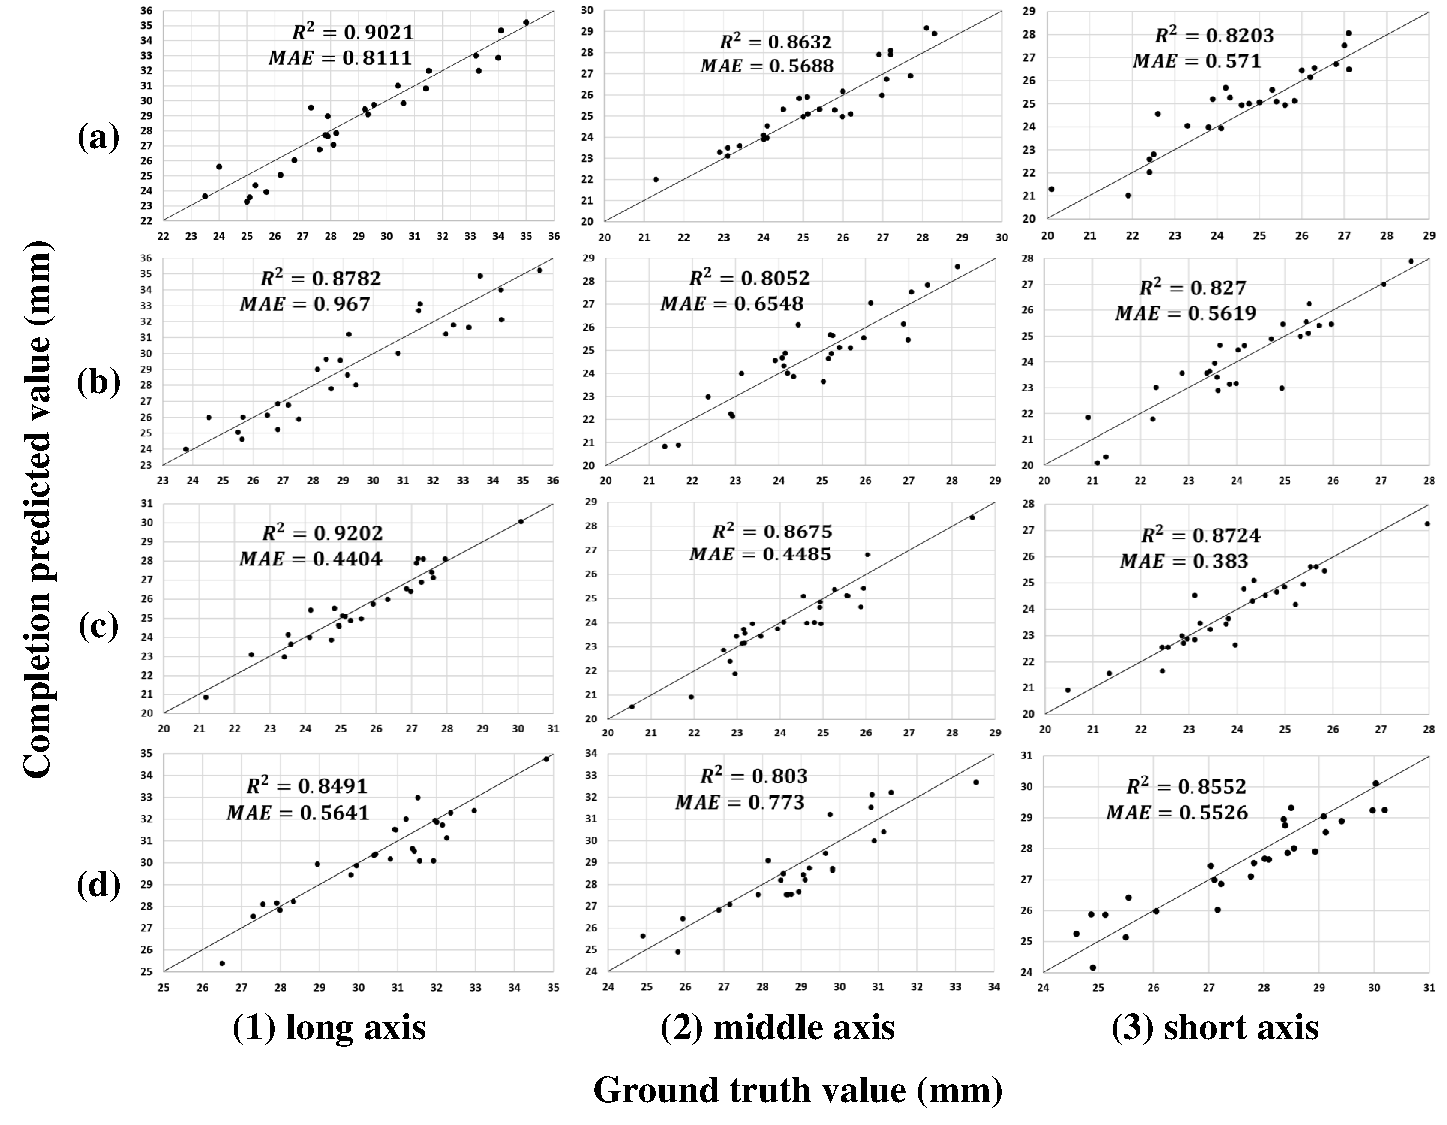
\includegraphics[width=1\textwidth]{figures/Figure14.pdf}
    \caption{Experimental results of axis length calculation for four species of fresh grape. From (a)-(d): Red Grape, Green Grape, Kyoho Grape, and Shine-Muscat Grape, and from (1)-(3): the calculation of the long, middle, and short axis, respectively.}
    \label{fig:raw16}
\end{figure}

As shown in Figure~\ref{fig:raw17}, each point on the subplot block represents a berry sample, the horizontal coordinate indicates the true value of the axis length, the vertical coordinate indicates the prediction value, and the $R^2$ and MAE are displayed in the figure at the same time. 
From the results, it can be seen that the proposed method achieves an average $R^2$ of 0.86 for the three axis lengths of the four species of grape. 
The analysis based on different perspectives is as follows.

(1) The different species: Red Grape, Green Grape, Kyoho Grape, and Shine-Muscat Grape axis lengths predicted to reach an average $R^2$ of 0.86, 0.84, 0.89, and 0.84, respectively. 
Among them, Kyoho Grape achieves the best results due to its berries with spherical shapes that are not too densely clustered and the lower difficulty in berry completion and morphology fitting. 
Secondly, Red Grape and Green Grape both present a typical ellipsoid shape, but the latter is less precise than the former due to its greater ratio of long axis to short axis, which provides a more complex presentation. 
In addition, Shine-Muscat Grape has the lowest precision, which is due to the fact that its berry grows tightly and squeeze each other heavily, and the completion and fitting suffer from a loss of precision.

(2) The different axis: the average $R^2$ of the four species of grape are 0.89, 0.83, and 0.84 for the long, middle, and short axis, respectively. 
It can be seen that the prediction accuracy of the long axis is significantly higher than that of the others, in which the $R^2$ of Red Grape and Kyoho Grape reach 0.90 and 0.92, respectively, realizing a high accuracy. 
This is due to the fact that in berry completion and fitting, the long axis is the easiest to determine, with less fitting error compared to the other two axes.

The experimental results show that the proposed method has achieved high accuracy in the calculation of the radius of different grape species. 
In addition, based on the radius prediction results, the volume of all 108 berry samples is calculated in this paper, and the experimental results are shown in Figure~\ref{fig:raw18}.

% figure 18
\begin{figure}[hbt!]
    \centering
    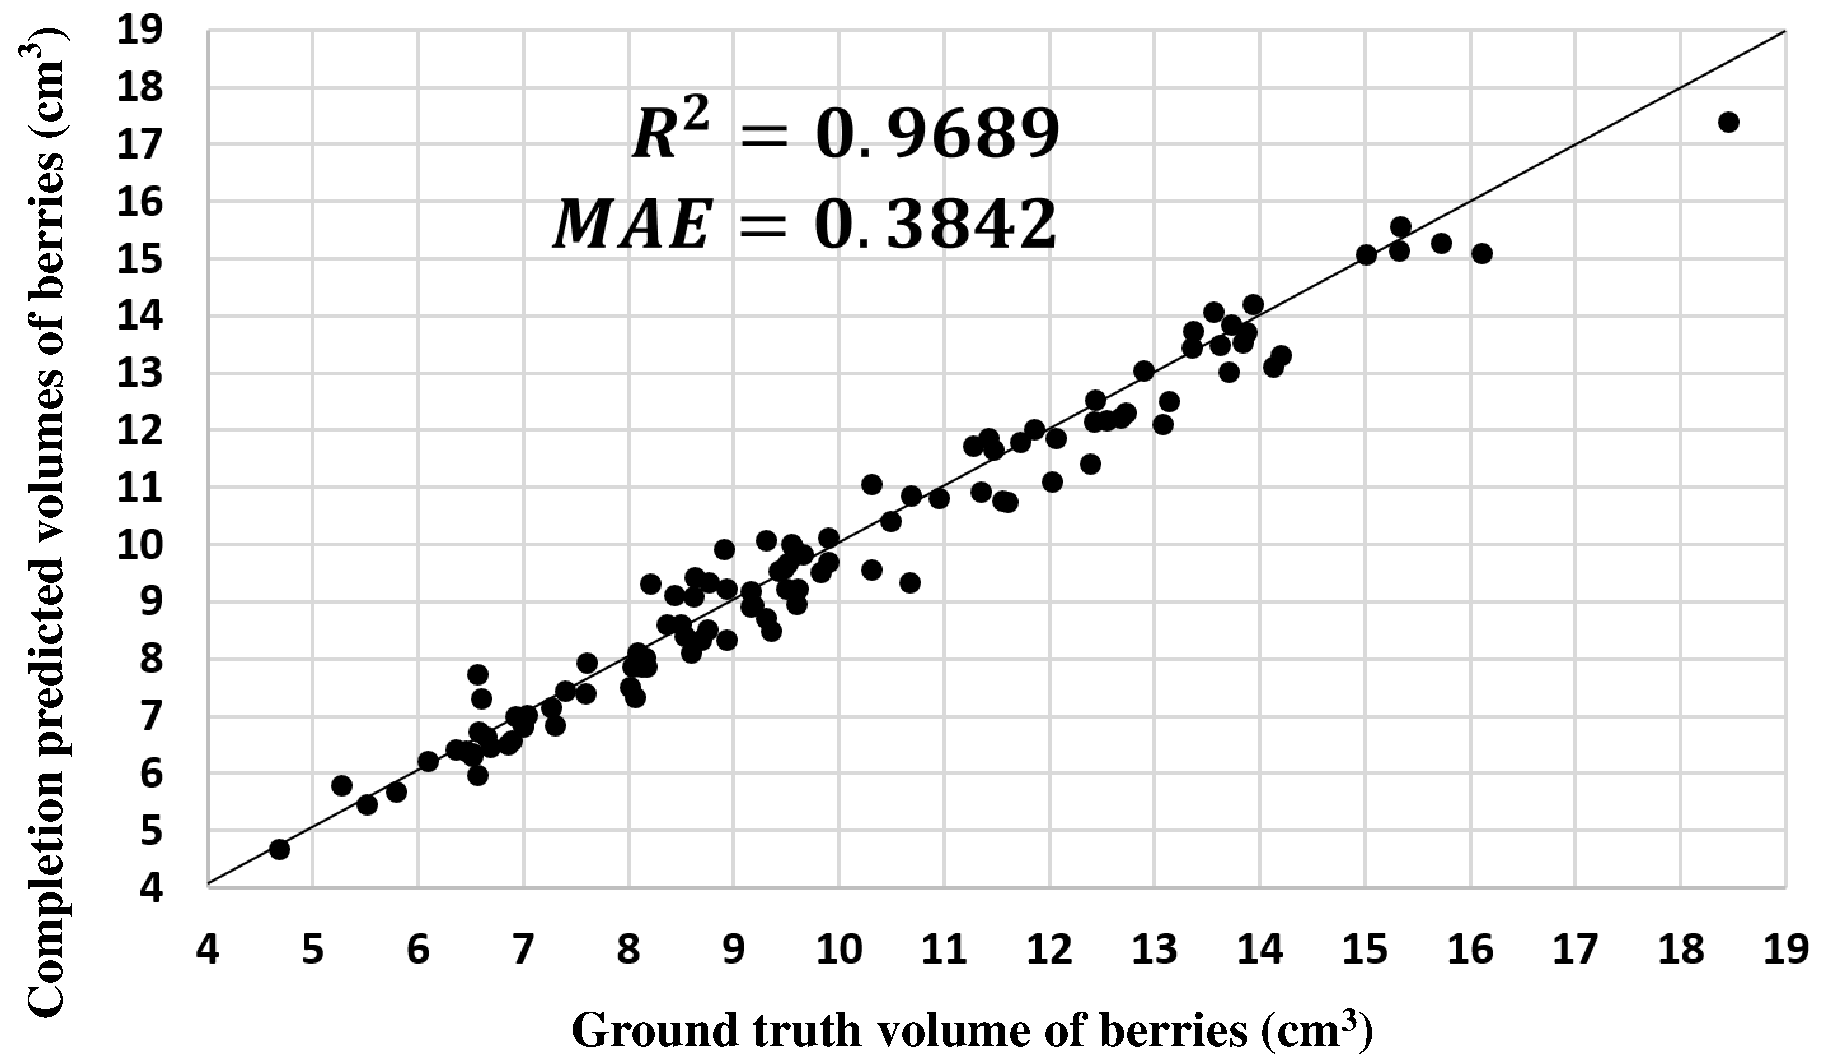
\includegraphics[width=1\textwidth]{figures/Figure15.pdf}
    \caption{Experimental results of berry volume calculation.}
    \label{fig:raw18}
\end{figure}

From the experimental results, it can be seen that the proposed method in the four species of berry volume phenotypic parameter calculation, $R^2$ reached 0.97, MAE is 0.3842 $cm^3$, with high precision, fully guarantee the accuracy of the prediction of the volume of different species.

\section{Discussion and Conclusion}

In this paper, a method for the automatic acquisition of 3D phenotypic parameters of grape is designed to address the problems of high labor cost, poor accuracy, and inability to realize end-to-end in the current work. 
Based on the point cloud of a bunch, the combination of deep learning point cloud processing algorithms realizes the counting of the number of berries, the calculation of berry radius, and berry volume. 
Moreover, to address the problem of incomplete surface of berry point cloud caused by occlusion, GrapeCPNet, a berry point cloud completion model based on the self-supervised training method, is designed to provide effective analytical data for berry-level phenotypic analysis.

At the same time, we found that GrapeCPNet is not effective in the case of complex berry appearance, such as drop-shaped. 
We have found that some researchers [45,46] have improved the completion effect by encoding a prior knowledge of the geometry of the object into the weights of the neural network. 
We subsequently consider utilizing the prior knowledge of berry geometry to achieve more detailed morphological feature extraction and representation to improve the quality of completion. 
In addition, the noise of data is also related to the effectiveness of the method proposed in this paper. 
How to implement the method in practical application scenarios, such as RGB-D collected point cloud data, is another issue to be considered in the future. 

Through the method proposed in this paper, the automated acquisition of 3D phenotypic parameters of grape can be realized, which is of great significance in the field of agricultural production and scientific research. 
First, there are large differences in berry morphology among different species of grape, and accurate reconstruction and analysis at the berry-level can help researchers analyze character differences more accurately. 
This plays an important role in breed improvement, cultivation management, and yield prediction. 
Secondly, the point cloud data analysis technology based on 3D reconstruction has a wide application prospect in the growth environment of field crops. 
Through the designed data acquisition method and related technologies, combined with the actual field crop growing environment, the growth process can be monitored and analyzed in real-time. 
Further, it can understand the phenotypic change law of crops under a natural growing environment better, provide a scientific basis for agricultural production, and optimize the production process and quality control.


\section*{CRediT authorship contribution statement}
\textbf{Wenli Zhang}: conceptualisation, methodology, supervision, funding acquisition, project administration, writing - review; \textbf{Chao Zheng}: methodology, software, data curation, writing - original draft \& editing; \textbf{Chenhuizi Wang}: data curation, software; \textbf{Pieter M. Blok}: methodology, supervision, writing - review \& editing; \textbf{Haozhou Wang}: methodology, writing - review \& editing; \textbf{Wei Guo}: conceptualisation, methodology, funding acquisition, supervision, writing - review \& editing.

\section*{Declaration of competing interest}
The authors declare that they have no known competing financial interests or personal relationships that could have appeared to influence the work reported in this paper.

\section*{Data availability}
The dataset, model weight and code will be made available on request.

\section*{Funding}
This study is partially funded by the ...

\section*{Acknowledgements}
We would like to thank ... \citep{blok_highthroughput_2025}

{\clearpage}

\bibliographystyle{elsarticle-harv}
\setcitestyle{aysep={}}
\bibliography{references}

\end{document}
